 \iffalse
\title{ME:2008}
\author{AI24BTECH11007}
\section{me}
\chapter{2008}
\fi


\item
	A set of $5$ jobs is to be processed on a single machine. The processing time (in days) is given in the table below. The holding cost for each job is Rs.$K$ per day.\\
		\begin{table}[ht]
\centering
\begin{tabular}{|c|c|}
\hline
\textbf{Job} & \textbf{Processing Time} \\ \hline
P            & 5                        \\ \hline
Q            & 2                        \\ \hline
R            & 3                        \\ \hline
S            & 2                        \\ \hline
T            & 1                        \\ \hline
\end{tabular}
\end{table}


		A schedule that minimizes the total inventory cost is 

		\hfill{(ME:2008)}
		\begin{multicols}{2}
			\begin{enumerate}
				\item T-S-Q-R-P
				\item P-R-S-Q-T
				\item T-R-S-Q-P
				\item P-Q-R-S-T
			\end{enumerate}
		\end{multicols}

    \item
        For generating a Coon's surface we require

		\hfill{(ME:2008)}
        \begin{enumerate}
            
            \item a set of grid points on the surface
            \item a set of grid control points
            \item four bounding curves defining the surface
            \item two bounding curves and a set of grid control points
        \end{enumerate}
    \item
        Internal gear cutting operation can be performed by

        \hfill{(ME:2008)}
        \begin{enumerate}
            \item milling
            \item shaping with rack cutter
            \item shaping with pinion cutter
            \item hobbing
        \end{enumerate}

 \item
        Consider the shaded triangular region $P$ shown in the figure. What is $\iint\limits_P xydxdy$?
        \vspace{0.2cm}
		\begin{center}
        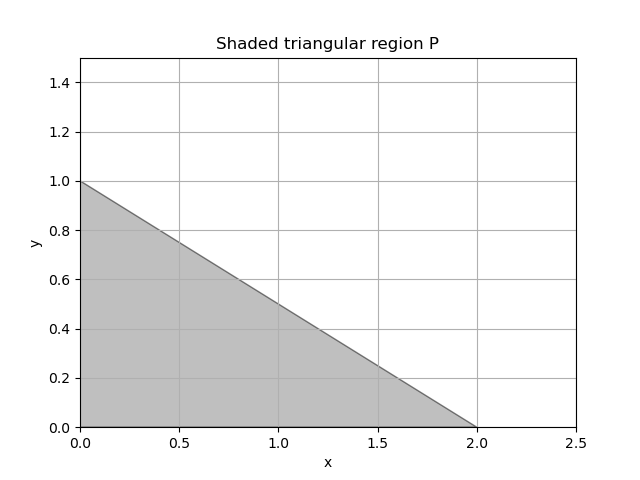
\includegraphics[width=0.4\textwidth]{figs/graphme8.png}
		\end{center}
        \vspace{0.2cm}

        \hfill{(ME:2008)}
        \begin{multicols}{4}
            \begin{enumerate}
                \item $\frac{1}{6}$
                \item $\frac{2}{9}$
                \item $\frac{7}{16}$
                \item $1$
            \end{enumerate}
        \end{multicols}
    
    \item 
        The directional derivative of the scalar function $f(x,y,z) = x^2 + 2y^2 + z$ at the point $P = (1,1,2)$ in the direction of the vector $\vec{a} = 3\hat{i} - 4\hat{j}$ is

        \hfill{(ME:2008)}
        \begin{multicols}{4}
            \begin{enumerate}
                \item $-4$
                \item $-2$
                \item $-1$
                \item $1$\\
            \end{enumerate}
        \end{multicols}

    \item
        For what value of $a$, if any, will the following system of equations in $x, y, z$ have a solution?
              
		\begin{align}
			2x + 3y &= 4 \\
			x + y + z &= 4 \\
			x + 2y - z &= a
                 \end{align}
               
        \hfill{(ME:2008)}
        \begin{multicols}{2}
            \begin{enumerate}
                \item Any real number
                \item $0$
                \item $1$
                \item There is no such value
            \end{enumerate}
        \end{multicols}
    
    \item
        Which of the following integrals is unbounded?

        \hfill{(ME:2008)}
        \begin{multicols}{2}
            \begin{enumerate}
                \item $\int_0^{\pi/4} \tan x \, dx$
                \item $\int_0^1 \frac{1}{x^2+1} \, dx$
                \item $\int_0^1 xe^{-x^2} \, dx$
                \item $\int_0^1 \frac{1}{1-x} \, dx$\\
            \end{enumerate}
        \end{multicols}

    \item
        The integral $\oint f(z) dz$ evaluated around the unit circle on the complex plane for $f(z) = \frac{\cos z}{z}$ is
       
       \hfill{(ME:2008)}
        \begin{multicols}{4}
            \begin{enumerate}
                \item $2\pi i$
                \item $4\pi i$
                \item $-2\pi i$
                \item $0$
            \end{enumerate}
        \end{multicols}
    
    \item
        The length of the curve $y = \frac{2}{3}x^{3/2}$ between $x=0$ and $x=1$ is

        \hfill{(ME:2008)}
        \begin{multicols}{4}
            \begin{enumerate}
                \item $0.27$
                \item $0.67$
                \item $1$
                \item $1.22$
            \end{enumerate}
        \end{multicols}
    
    \item
	The eigenvectors of the matrix \[\myvec
{1 & 2 \\ 0 & 2} \] are written in the form $\myvec{1\\a}$ and $\myvec{1\\b}.$ What is $a + b$?

        \hfill{(ME:2008)}
        \begin{multicols}{4}
            \begin{enumerate}
                \item $0$
                \item $\frac{1}{2}$
                \item $1$
                \item $2$
            \end{enumerate}
        \end{multicols}
                                  
    \item 
	Let $f = x^y$. What is $\frac{\partial^2 f}{\partial x \partial y}$ at $x = 2$, $y = 1$?

	 \hfill{(ME:2008)}

    \begin{multicols}{4}
        \begin{enumerate}
            \item 0
            \item ln 2
            \item 1
            \item $\frac{1}{\ln 2}$
        \end{enumerate}
    \end{multicols}

    \item 
	    It is given that $y^{\prime \prime} + 2y^\prime + y = 0, y(0) = 0, y(1) = 0$. What is $y(0.5)$?

	     \hfill{(GATE-ME:2008)}

    \begin{multicols}{4}
        \begin{enumerate}
            \item 0
            \item 0.17
            \item 0.62
            \item 1.13
        \end{enumerate}
    \end{multicols}

    \item The strain energy stored in the beam with flexural rigidity $EI$ and loaded as shown in the figure is
	    \begin{center}
	    \begin{tikzpicture}

% Draw the beam
\draw (0,0) -- (6,0); % Horizontal beam

% Supports
\draw (0,0) node[ground, rotate=90]{};   % Pin support on the left
\draw (6,0) circle (3pt);                % Roller support on the right

% Load points and forces
\draw[thick, ->] (2,0.5) -- (2,0); % Force P at 2L from the left
\draw[thick, ->] (4,0.5) -- (4,0); % Force P at 2L from the right

% Labels
\node at (2,0.7) {$P$}; % Label for the first force
\node at (4,0.7) {$P$}; % Label for the second force
\node at (1, -0.3) {$L$}; % Left distance label
\node at (5, -0.3) {$L$}; % Right distance label
\node at (3, -0.3) {$2L$}; % Middle distance label

% Dashed lines for distances
\draw[dashed] (2,0) -- (2,-0.7); % Left force vertical line
\draw[dashed] (4,0) -- (4,-0.7); % Right force vertical line

% Distance labels
\draw[<->] (0,-0.5) -- (2,-0.5);
\draw[<->] (2,-0.5) -- (4,-0.5);
\draw[<->] (4,-0.5) -- (6,-0.5);

\end{tikzpicture}


	    \end{center}
 
 \hfill{(ME:2008)}
 \begin{multicols}{2}
	 \begin{enumerate}
	    \item $\frac{P^2 L^3}{3EI}$
            \item $\frac{2P^2 L^3}{3EI}$
            \item $\frac{4P^2 L^3}{3EI}$
            \item $\frac{8P^2 L^3}{3EI}$
	    
        \end{enumerate}
    \end{multicols}

    \item For the component loaded with a force $F$ as shown in the figure, the axial stress at the corner point $P$ is
	    \begin{center}
	    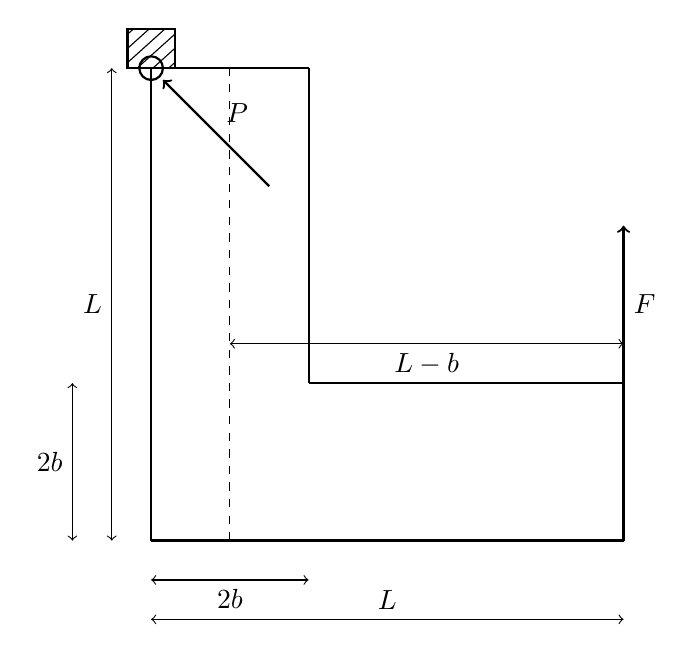
\begin{tikzpicture}

    % Draw the L-shaped structure
    \draw[thick] (0,0) -- (0,6); % vertical part
    \draw[thick] (0,0) -- (6,0); % top horizontal part
    \draw[thick] (0,6) -- (2,6); % downward part
    \draw[thick] (2,2) -- (6,2); % bottom horizontal part
    \draw[thick] (2,2) -- (2,6); % vertical part
	\draw[thick] (6,0) -- (6,2);

    % Draw the wall (left)
  \begin{scope}
    % Clip to the shape
    \clip (-0.3,6) rectangle (0.3,6.5);
    % Draw diagonal lines
    \foreach \x in {-6,-5.8,...,6} { % Adjust spacing by modifying the range
        \draw[thin] (\x,5.8) -- (\x+1,6.7); % Adjust the angle and range as needed
    }
\end{scope}

% Outline the shape
\draw[thick] (-0.3,6.5) -- (0.3,6.5) -- (0.3,6) -- (-0.3,6) -- cycle;

    % Draw hinge circle at the corner
    \draw[thick] (0,6) circle (0.15);

    % Forces
    \draw[thick,->] (6,2) -- (6,4) node[midway, right] {$F$}; % Force F
    \draw[thick,<-] (0.15,5.85) -- (1.5,4.5) node[midway, above right] {$P$}; % Force P

    % Dimensions
    \draw[<->] (-0.5,0) -- (-0.5,6) node[midway, left] {$L$}; % Left dimension L
    \draw[<->] (0,-0.5) -- (2,-0.5) node[midway, below] {$2b$}; % Bottom dimension 2b
    \draw[<->] (1,2.5) -- (6,2.5) node[midway, below] {$L-b$}; % Middle dimension L-b
    \draw[<->] (0,-1) -- (6,-1) node[midway, above] {$L$}; % Right dimension L
	\draw[<->] (-1,0) -- (-1,2) node[midway, left] {$2b$};
    
    % Dashed line (center axis for the square at the bottom)
    \draw[dashed] (1,0) -- (1,6);

   \end{tikzpicture}

	    \end{center}

	     \hfill{(ME:2008)}

       \begin{multicols}{4}
        \begin{enumerate}
            \item $\frac{F(3L-b)}{4b^3}$
            \item $\frac{F(3L+b)}{4b^3}$
            \item $\frac{F(3L-4b)}{4b^3}$
            \item $\frac{F(3L-2b)}{4b^3}$
        \end{enumerate}
    \end{multicols}

    \item A solid circular shaft of diameter 100 mm is subjected to an axial stress of 50 MPa. It is further subjected to a torque of 10 kNm. The maximum principal stress experienced on the shaft is closest to

	     \hfill{(ME:2008)}

    \begin{multicols}{4}
        \begin{enumerate}
            \item 41 MPa
            \item 82 MPa
            \item 164 MPa
            \item 204 MPa
        \end{enumerate}
    \end{multicols}

    \item A circular disk of radius $R$ rolls without slipping at a velocity $v$. The magnitude of the velocity at point $P$ is\\
	    \begin{center}
	    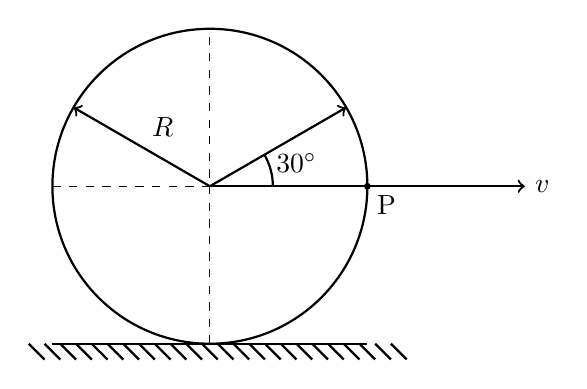
\begin{tikzpicture}

% Draw the circle
\draw[thick] (0,0) circle(2);

% Draw the horizontal and vertical dashed lines
\draw[dashed] (-2,0) -- (2,0);
\draw[dashed] (0,-2) -- (0,2);

% Draw the radius R and the angle 30 degrees
\draw[thick,->] (0,0) -- (-1.73,1) node[midway, above right] {$R$};
\draw[thick] (0,0) -- (2,0) node[midway, below] {};
\draw[thick,->] (2,0) -- (4,0) node[right] {$v$};
\draw[thick,->] (0,0) -- (1.73,1);

% Draw point P and label
\filldraw (2,0) circle (1pt) node[below right] {P};

% Angle marker
\draw[thick] (0.8,0) arc[start angle=0, end angle=30, radius=0.8];
\node at (1.1,0.3) {$30^\circ$};

% Draw the ground
\draw[thick] (-2,-2) -- (2,-2);
\draw[thick] (-2.3,-2) -- (-2.1,-2.2);
\draw[thick] (-2.1,-2) -- (-1.9,-2.2);
\draw[thick] (-1.9,-2) -- (-1.7,-2.2);
\draw[thick] (-1.7,-2) -- (-1.5,-2.2);
\draw[thick] (-1.5,-2) -- (-1.3,-2.2);
\draw[thick] (-1.3,-2) -- (-1.1,-2.2);
\draw[thick] (-1.1,-2) -- (-0.9,-2.2);
\draw[thick] (-0.9,-2) -- (-0.7,-2.2);
\draw[thick] (-0.7,-2) -- (-0.5,-2.2);
\draw[thick] (-0.5,-2) -- (-0.3,-2.2);
\draw[thick] (-0.3,-2) -- (-0.1,-2.2);
\draw[thick] (-0.1,-2) -- (0.1,-2.2);
\draw[thick] (0.1,-2) -- (0.3,-2.2);
\draw[thick] (0.3,-2) -- (0.5,-2.2);
\draw[thick] (0.5,-2) -- (0.7,-2.2);
\draw[thick] (0.7,-2) -- (0.9,-2.2);
\draw[thick] (0.9,-2) -- (1.1,-2.2);
\draw[thick] (1.1,-2) -- (1.3,-2.2);
\draw[thick] (1.3,-2) -- (1.5,-2.2);
\draw[thick] (1.5,-2) -- (1.7,-2.2);
\draw[thick] (1.7,-2) -- (1.9,-2.2);
\draw[thick] (1.9,-2) -- (2.1,-2.2);
\draw[thick] (2.1,-2) -- (2.3,-2.2);
\draw[thick] (2.3,-2) -- (2.5,-2.2);

\end{tikzpicture}

	    \end{center}

	     \hfill{(ME:2008)}

       \begin{multicols}{4}
        \begin{enumerate}
            \item $\frac{\sqrt{3}}{v}$
            \item $\frac{\sqrt{3} v}{2}$
            \item $\frac{v}{2}$
            \item $v \sqrt{3}$
        \end{enumerate}
    \end{multicols}

    \item Consider a truss PQR loaded at $P$ with a force $F$ as shown in the figure. The tension in the member $QR$ is\\
	    \begin{center}
	    \begin{tikzpicture}

% Define points
\coordinate (Q) at (0,0);
\coordinate (R) at (6,0);
\coordinate (P) at (3,3);

% Draw the truss members
\draw[thick] (Q) -- (P) -- (R);
\draw[thick] (Q) -- (R);

% Draw the force F
\draw[thick,<-] (P) -- +(0,2) node[above] {$F$};

% Draw support at Q (hinged)
\draw[thick] (Q) -- +(-0.5,-0.5);
\draw[thick] (Q) -- +(0.5,-0.5);
\draw[thick] (Q) -- +(0,-0.7);

% Draw support at R (roller)
\draw[thick] (R) -- +(0,-0.5);
\draw[thick] (R) -- +(0.5,-0.5);
\draw[thick] (R) -- +(0,-0.7);
\draw[thick] (R) -- +(-0.5,-0.5);

% Add angle markers
\draw[thick] (0.5,0) arc[start angle=0,end angle=45,radius=0.5];
\node at (0.8,0.25) {$45^\circ$};

\draw[thick] (5.5,0) arc[start angle=180,end angle=150,radius=0.8];
\node at (5,0.25) {$30^\circ$};

% Label points
\node at (Q) [left] {$Q$};
\node at (R) [right] {$R$};
\node at (P) [above left] {$P$};

\end{tikzpicture}

	    \end{center}

	     \hfill{(ME:2008)}

       \begin{multicols}{4}
        \begin{enumerate}
            \item $0.5F$
            \item $0.63F$
            \item $0.73F$
            \item $0.87F$
        \end{enumerate}
    \end{multicols}



